% Verschiebung von Koordinatensystemen © 2022 by Justus John Michael Seeck
% is licensed under Attribution-NonCommercial-ShareAlike 4.0 International
% A copy of this license is available at https://creativecommons.org/licenses/by-nc-sa/4.0/
\documentclass{article}

% Umlaut-Support
\usepackage[ngerman]{babel}
\usepackage[utf8]{inputenc}
\usepackage[T1]{fontenc}

% AMS
\usepackage{amsmath}
\usepackage{amssymb}
\usepackage{amsthm}

% Koordinatensysteme
\usepackage{tkz-euclide}

% Grafiken und Bilder
\usepackage{graphicx}

% Gradsymbol etc.
\usepackage{gensymb}

% Links
\usepackage[colorlinks=true,linkcolor=black,anchorcolor=black,citecolor=black,filecolor=black,menucolor=black,runcolor=black,urlcolor=black]{hyperref}

% Seiteneinrichtung
\usepackage[a4paper, left=3cm, right=3cm, top=3cm, bottom=3cm]{geometry} % https://latex-kurs.blogspot.com/2012/09/latex-seitenrander-und-textwidth.html

% Befehle
\newcommand{\m}[1]{\begin{pmatrix}#1\end{pmatrix}}


\newcommand{\myeq}[1]{\mathrel{\overset{\makebox[0pt]{\mbox{\normalfont\tiny\sffamily #1}}}{=}}}

% Einstellungen
\setlength{\parindent}{0pt}

% Metadaten
\title{Verschiebung von Koordinatensystemen}
\author{Justus John Michael Seeck}
\date{\today}

% Dokumentenbeginn
\begin{document}
    \maketitle

    \tableofcontents

    \newpage

    \section{Einführung}

    \subsection{Vorwort}

    In der folgenden Arbeit wird lediglich die Verschiebung von Koordinatensystemen in der Ebene (also in zwei Dimensionen) behandelt.
    Die Methodik lässt sich jedoch auch auf die dritte Dimension übertragen. Auch die Anzahl der Verschiebungen ist
    beliebig, da man die
    hier verwendete Formel beliebig oft hintereinander anwenden kann. Es wird sich hier jedoch auf eine Verschiebung beschränkt.
    Die Verschiebung von Koordinatensystemen findet beispielweise in der Robotik Anwendung. Am Ende eines Roboterarms,
    welcher sich beeits in einem Koordinatensystem befindet,
    befindet sich meist ein weiteres Koordinatensystem,
    "Toolsystem". In diesem System gibt es keine Verschiebung der einzelnen Punkte, wenn sich der Arm bewegt,
    sondern lediglich wenn sich das Tool, oder dessen Ladung beziehungsweise Werkzeug bewegt.

    \subsection{Schreibweisen und Definitionen}
    
    \paragraph{Punkte}

    Ein Punkt $P$ wurde bisher in der Form $P(x|y)$ dargestellt. Dies wird in der folgenden Arbeit nicht mehr verwendet. Stattdessen wird
    der Punkt $P$ in der Form $\m{x \\ y}$ dargestellt. Dies ist eine sogenannte Matrix mit zwei Zeilen und einer Spalte.
    Die erste Zeile enthält die x-Koordinate, die zweite Zeile die y-Koordinate.
    Da im folgenden mit zwei verschiedenen Koordinatensystemen, dem Weltsystem oder Ursprungssystem $U$
    und dem Toolsystem $T$, gearbeitet wird,
    werden Punkte im Bezug auf ein Koordinatensystem mit Index angegeben, insofern dies nötig ist.
    Der Punkt $P$ im Bezug zum Weltsystem $U$ wird
    folgendermaßen dargestellt: ${[P]}_{U}$.
    Im Bezug zum Toolsystem lautet die Darstellung ${[P]}_{T}$.
    Die Darstellung kann auch ohne eckige Klammern erfolgen.
    Punkte haben dann lediglich einen Index, der das Koordinatensystem angibt.
    
    \section{Vektoren}

    Geometrische Vektoren sind Pfeile. $\vec{v}$ ist ein Vektor.
    Vektoren werden durch ihre Länge in $x$-Richtung und $y$-Richtung definiert
    (bei drei Dimensionen zusätzlich in $z$-Richtung) und mit einem Pfeil über dem Buchstaben gekennzeichnet.
    Vektoren haben keine Feste Postition im Koordinatensystem. Sie können beliebig verschoben werden.
    Solange der Vektor alle seine Eigenschaften (Länge in $x$-, $y$- und ggf. $z$-Richtung) behält,
    ist er der gleiche Vektor. \textbf{Anhang: Vektoren 1}. Zwischen zwei gleichen Vektoren lässt sich ein
    Paralellogramm zeichnen.
    

    \subsection{Rechnen mit Vektoren und Punkten}
    Vektoren können durch mathematische Operationen verändert werden. 
    Sie können addiert, subtrahiert und mit einem Skalar (einer Zahl) multipliziert werden.
    \textbf{Anhang: Vektoren 2}.
    Es sind folgende Regeln gültig:


    \textbf{Summen}
    \[
        \begin{split}
            \m{a \\ b} + \m{c \\ d} = \m{a+c \\ b+d}
        \end{split}
    \]

    \textbf{Differenzen}
    \[
        \begin{split}
            \m{a \\ b} - \m{c \\ d} = \m{a-c \\ b-d}
        \end{split}
    \]

    \textbf{(Skalares) Produkt} (Erklärung folgt)
    \[
        \begin{split}
            r \cdot \m{a \\ b} = \m{r \cdot a \\ r \cdot b}
        \end{split}
    \]

    Aus der Grafik (\textbf{Anhang: Vektoren 2}) wird zudem deutlich, dass die Summe zweier Vektoren (eine Aneinanderlegung von Pfeilen)
    die Summe der beiden Einzelvektoren (Koordinatenvektoren) ist:

    \[
        \begin{split}
            [\vec{w} + \vec{a}] = [\vec{w}] + [\vec{a}]
        \end{split}
    \]

    Punkte können mithilfe von Vektoren verschoben werden. Der Punkt wird dabei mit dem Vektor
    addiert. Dies entspricht dem Anhängen des Vektors an den Punkt. Das Ende des Vektors entspricht dann
    der Koordinate des verschoben Punkts. Man kann auch ein Parallelogramm zwischen dem Punkt und dem
    Vektor bilden. Der fehlende Punkt
    ergibt dann die gesuchte Stelle des neuen Punktes. \textbf{Anhang: Vektoren 3}.

    \subsection{Einheitsvektoren im Koordinatensystem}
    Ein Punkt $P$ kann mit Hilfe von Einheitsvektoren im Koordinatensystem $U$ beschrieben werden.
    Das Koordinatensystem $U$ hat rechtwinklige Achsen.
    Bei einer Drehung der $x$-Achse um 90 Grad gegen den Uhrzeigersinn entsteht deswegen die $y$-Achse.
    Es gibt jeweils einen Einheitsvektor in
    $x$-Richtung und einen Einheitsvektor in $y$-Richtung (bei drei Dimensionen zusätzlich in $z$-Richtung).
    Der Einheitsvektor in $x$-Richtung ist $\vec{{x}_{U}} = \m{1 \\ 0}$ und der Einheitsvektor in
    $y$-Richtung ist $\vec{{y}_{U}} = \m{0 \\ 1}$ (Es sind auch andere Bezeichnungen / Buchstaben für Einheitsvektoren
    möglich).
    Die Länge des Einheitsvektors ist dabei $1$
    (eine Längeneinheit)
    in seine respective Richtung. Um nun beispielweise den Punkt
    ${[P]}_{U} = \m{a \\ b}$ zu beschreiben, benötigt man den Ursprung des Koordinatensystems ${O}_{U}$, seine Koordinate in $x$-Richtung (hier: $a$),
    seine Koordinate in $y$-Richtung (hier: $b$) und die beiden Einheitsvektoren $\vec{{x}_{U}}$ und $\vec{{y}_{U}}$.
    
    Es ergibt sich die folgende Formel:

    \[
        \begin{split}
            {[P]}_{U} = {[O]}_{U} + a \cdot \vec{{x}_{U}} + b \cdot \vec{{y}_{U}} = \m{a \\ b}
        \end{split}
    \]

    Der Punkt ${[P]}_{U}$ entspricht dem dem Punkt ${[O]}_{U}$ zu dem man eine Verschiebung in
    $x$-Richtung (hier: $a \cdot \vec{{x}_{U}}$) und $y$-Richtung (hier: $b \cdot \vec{{y}_{U}}$) hinzufügt.
    \textbf{Anhang: Vektoren 4}.

    Befindet sich ein Vektor in einem Koordinatensystem, lässt sich dieser durch die Differenz
    des Anfangs- und Endpunktes des Vektors darstellen.
    Es ergibt sich folgendes: 
    % https://youtu.be/QHywLVUK3hc?t=1840
    \[
        \begin{split}
            \vec{v} = \m{\Delta{x} \\ \Delta{y}}
        \end{split}
    \]

    \textbf{Anhang: Vektoren 5} zeigt die Darstellung eines Vektors in einem Koordinatensystem.
    

    \section{Die Verschiebung von Koordinatensystemen}
    
    Unser Ziel besteht darin, die bekannten Koordinaten eines Objekts, beispielweise eines Punktes
    im Toolsystem $T$ in das Koordinatensystem $U$ zu überführen.
    Dazu benötigen wir die Verschiebung des Ursprungs des Toolsystems ${[{O}_{T}]}_{U}$ ausgehend vom 
    Ursprung des Koordinatensystems ${[O]}_{U}$ im Bezug auf das Ursprungssystem.
    Diese Verschiebung kann durch einen Vektor beschrieben werden.
    Dieser Vektor wird als Verschiebevektor bezeichnet.

    % Anhang: Bild mit zwei Koordinatensystemen, den Einheitsvektoren und Ursprüngen. Zusätzlich: Drehung

    Die Position von ${[{O}_{T}]}_{U}$ ist gegeben.

    \subsection{Länge von Vektoren und Abstände von Punkten}
    Um den Verschiebevektor zu bestimmen, der Vektor, um den der Punkt $O_U$ verschoben werden muss,
    um zum Punkt ${[{O}_{T}]}_{U}$ zu gelangen, 
    wird der Abstand zwischen dem Ursprung
    des Toolsystems ${[{O}_{T}]}_{U}$ und dem Ursprung des Koordinatensystems $U$ benötigt,
    also ${[O]}_{U}$. Diese Formel kann auch für andere Punkte angewendet werden.
    
    Die Länge eines Vektors wird durch die Pythagoras-Formel berechnet.
    Die Länge von $\vec{v}$ wird folgendermaßen dargestellt $\lVert \vec{v} \rVert$. 
    

    \[
        \begin{split}
            \lVert \vec{v} \rVert &= \left \lVert \m{\Delta x \\ \Delta y} \right \rVert \\
            \lVert \vec{v} \rVert &= \sqrt{\Delta{x}^2 + \Delta{y}^2}
        \end{split}
    \]

    Der Abstand zwischen den Punkten $P$ und $Q$ ist nach dieser Formel dann:
    $dist(P, Q) = \lVert \vec{PQ} \rVert$.
    
    ist ${[P]}_{U} = \m{u_x \\ u_y}$ und ${[Q]}_{U} = \m{v_x \\ v_y}$, dann folgt:

    \[
      \begin{split}
        dist(P, Q) &= \lVert \vec{PQ} \rVert \\
        &= \left \lVert \m{v_x - u_x \\ v_y - u_y} \right \rVert \\
        &= \sqrt{(v_x - u_x)^2 + (v_y - u_y)^2} \\
      \end{split}  
    \] 

    \subsection{Das Skalarprodukt}
    
    "Das Skalarprodukt ist eine mathematische Verknüpfung, die zwei Vektoren eine Zahl (Skalar) zuordnet."

    (https://www.mathebibel.de/skalarprodukt - Letzter Aufruf: 26.12.2022 @ 17:03:54)
    In diesem Fall wird das Skalarprodukt verwendet, um den Winkel $\theta$ zwischen zwei Vektoren zu berechnen.
    \textbf{Anhang: Skalarprodukt 1} zeigt eine Skizze.
    
    $\theta$ ist der Winkel zwischen den Vektoren $\vec{v}$ und $\vec{u}$.
    Beide Vektoren haben den selben Ursprung. Der Winkel $\theta$ ist hierbei ungerichtet
    (Siehe \textbf{Anhang: Skalarprodukt 1}) und liegt zwischen 0 und 180 Grad.
    
    Der kosinussatz besagt nun folgendes:

    \[
        \begin{split}
            \lVert \vec{v} - \vec{u} \rVert &= \lVert \vec{u} \rVert ^2 + \lVert \vec{v} \rVert - 2 \cdot \lVert \vec{u} \rVert \cdot \lVert \vec{v} \rVert \cdot \cos \theta \\
        \end{split}  
    \]

    Aus dem Kosinussatz folgt das Skalarprodukt von $\vec{u}$ und $\vec{v}$:

    \[
        \begin{split}
            \frac{1}{2} \cdot \left ( \lVert \vec{u} \rVert ^2 + \lVert \vec{v} \rVert ^2 - \lVert \vec{v} - \vec{u} \rVert ^2 \right ) &= \lVert \vec{u} \rVert \cdot \lVert \vec{v} \rVert \cdot \cos \theta \\
            &= \langle \vec{u} \vert \vec{v} \rangle \\
        \end{split}  
    \]

    In Koordinaten lässt sich das Skalarprodukt wie folgt darstellen.

    Gegeben sind:
    ${\vec{u}}_{s} = \m{u_x \\ u_y}$, ${\vec{v}}_{s} = \m{v_x \\ v_y}$

    \[
        \begin{split}
            \left \langle \m{u_x \\ u_y} \vert \m{v_x \\ v_y} \right \rangle \myeq{Def.} \left \langle \vec{u} \vert \vec{v} \right \rangle = \frac{1}{2} \cdot \left ( \lVert \m{u_x \\ u_y} \rVert ^2 + \lVert \m{v_x \\ v_y} \rVert ^2 - \lVert \m{v_x - u_x \\ v_y - u_y} \rVert ^2 \right ) \\
            = \frac{1}{2} \cdot \left ( u_x^2 + u_y^2 + v_x^2 + v_y^2 - [(v_x - u_x)^2 + (v_y - u_y)^2] \right ) \\
        \end{split}
    \]

    Anwendung der binomioschen Formeln und anschließendes vereinfachen ergibt:

    \[
      \begin{split}
        &= \frac{1}{2} \cdot \left ( u_x^2 + u_y^2 + v_x^2 + v_y^2 - [u_x^2 + v_x^2 - 2u_x v_x + u_y^2 + v_y^2 - 2u_y v_y] \right ) \\
        &= \left \langle \m{u_x \\ u_y} \vert \m{v_x \\ v_y} \right \rangle \\
        &= u_x v_x + u_y v_y
      \end{split}  
    \]

    Es ist zu beachten, dass sich das Skalarprodukt nur mit Vektoren (Pfeilen) bilden lässt.
    Es ist nicht möglich, das Skalarprodukt mit Punkten zu bilden.


    Nun lässt sich durch Umstellen der Winkel zwischen zwei koordinatengegebenen
    Vektoren ($\vec{u}$ und $\vec{v}$) berechnen:

    Aus den oberen Gleichungen geht hervor:

    \[
      \begin{split}
        \langle \vec{u} \vert \vec{v} \rangle &= \lVert \vec{u} \rVert \cdot \lVert \vec{v} \rVert \cdot \cos \theta \\
        &= \left \langle \m{u_x \\ u_y} \vert \m{v_x \\ v_y} \right \rangle \\
        &= u_x v_x + u_y v_y \\
      \end{split}  
    \]

    mit $\lVert \vec{u} \rVert = \sqrt{u_x^2 + u_y^2}$ und $\lVert \vec{v} \rVert = \sqrt{v_x^2 + v_y^2}$, dass $\theta$ zwischen 0 und 180 Grad folgendes Ergibt:
     
    \[
      \begin{split}
        \cos \theta &= \frac{\langle \vec{u} \vert \vec{v} \rangle}{\lVert \vec{u} \rVert \cdot \lVert \vec{v} \rVert} \\
        \theta &= \cos^{-1} \left ( \frac{\langle \vec{u} \vert \vec{v} \rangle}{\lVert \vec{u} \rVert \cdot \lVert \vec{v} \rVert} \right ) \\
      \end{split}  
    \]

    \subsection{Koordinaten Transformieren}

    Es wird ein wie in Punkt 2.2 beschriebenes Koodinatensystem $T$ auf ein anderes Koordinatensystem $U$ gelegt.
    Im Toolsystem $T$ wird ein Punkt $P$ durch Koordinaten beschrieben.
    Das Ziel ist, die Koordinaten des Punktes $P$ im Toolsystem $U$ mathematisch zu bestimmen.

    Das Skalarprodukt der beiden Koordinatenvektoren ergibt $0$, da die beiden Vektoren senkrecht zueinander stehen.

    Wie bereits in Punkt 2.2 beschrieben, lassen sich Punkte so mit Hilfe der Einheitsvektoren
    beschreiben. \textbf{Anhang: Koordinatentransformation 1}

    Formel:

    \[
        \begin{split}
            {[P]}_{U} = {[O]}_{U} + a \cdot \vec{{x}_{U}} + b \cdot \vec{{y}_{U}} = \m{a \\ b}
        \end{split}
    \]

    Ist der Verschiebevektor (also der Vektor von $O_U$ zu $O_T$) bekannt,
    so kann die Formel wie folgt umgeschrieben werden:

    \[
        \begin{split}
            \vec{u} = \Delta x \cdot \vec{{x}_{U}} + \Delta y \cdot \vec{{y}_{U}} = \m{\Delta x \\ \Delta y}
        \end{split}
    \]

    ${[P]}_{T}$ wird durch $\m{x_T \\ y_T}$ beschrieben. $P$ wird folgendermaßen in $U$ beschrieben:

    \[
        \begin{split}
            {[P]}_{U} &= {\left [{O}_{T} + {x}_{T} \cdot \vec{a}_T + {y}_{T} \cdot \vec{b}_T \right ]}_{U} \\
            &= {[O_T]}_{U} + x_T \cdot {[\vec{a}_T]}_U + y_T \cdot {[\vec{b}_T]}_U \\
        \end{split}
    \]

    Um die Koordinaten des Punktes ${[P]}_U$ zu bestimmen, reicht es, wie in der oberen Gleichung erkenntlich wird,
    ${[O_T]}_{U}$, ${[\vec{a}_T]}_U$ und ${[\vec{b}_T]}_U$ zu bestimmen.

    \subsection{Anwendung}

    Gegeben sind ${[P]}_T = \m{x_T \\ y_T}$, ${[O_T]}_{U} = \m{x_{OTU} \\ y_{OTU}}$ und der Drehwinkel $\alpha$.
    
    Die Einheitsvektoren bezüglich des Toolsystems $T$ lassen sich mit Hilfe von Sinus und Cosinus berechnen:

    \[
        \begin{split}
            {[\vec{a}_T]}_U = \m{\cos \alpha \\ \sin \alpha} \\
            {[\vec{b}_T]}_U = \m{\cos \alpha + 90 \degree \\ \sin \alpha + 90 \degree} \\
        \end{split}
    \]

    Durch das Skalarprodukt $\left \langle \vec{a}_T \Vert \vec{b}_T \right \rangle$ kann das erhaltene Ergebnis
    auf Korrektheit überpräft werden. Das Ergebnis des Skalarprodukts muss 0 sein, da beide Vektoren trotz der Drehung
    senkrecht zueinander stehen. Die länge der Einzelnen Vektoren muss ebenfalls 1 betragen. 

    \[
        \begin{split}
            {[P]}_{U} &= {[O_T]}_{U} + x_T \cdot {[\vec{a}_T]}_U + y_T \cdot {[\vec{b}_T]}_U \\
            &= \m{x_{OTU} \\ y_{OTU}} + x_T \cdot \m{\cos \alpha \\ \sin \alpha} + y_T \cdot \m{\cos \alpha + 90 \degree \\ \sin \alpha + 90 \degree} \\
            &= \m{x_{OTU} + x_T \cdot \cos \alpha + y_T \cdot \cos \alpha + 90 \degree \\ y_{OTU} + x_T \cdot \sin \alpha + y_T \cdot \sin \alpha + 90 \degree} \\
        \end{split}
    \]

    Diese Gleichung liefert bereits das korrekte Ergebnis. Es gibt jedoch eine Möglichkeit, die Gleichung zu vereinfachen.
    Dafür wird die sogenannte Matrizenrechnung verwendet.

    \subsection{Matrizenrechnung}

    Eine Matrix ist ein rechteckiges Zahlenschema.
    $M = \m{\frac{1}{\sqrt{2}} & \frac{-1}{\sqrt{2}} \\ \frac{1}{\sqrt{2}} & \frac{1}{\sqrt{2}}}$ ist eine Matrix
    mit zwei Zeilen und zwei Spalten.

    Durch Matzizen lässt sich die obige Gleichung folgendermaßen vereinfachen.

    Da $\cos \alpha + 90 \degree = - \sin \alpha$ und $\sin \alpha + 90 \degree = \cos \alpha$ gilt,
    kann die Matrix wie folgt definiert werden:

    \[
        \begin{split}
            M = \m{\cos \alpha & - \sin \alpha \\ \sin \alpha & \cos \alpha}
        \end{split}
    \]

    $x_T$ und $y_T$ werden dann mit der Matrix multipliziert:

    \[
        \begin{split}
            {[P]}_{T} \cdot M = \m{x_T \\ y_T} \cdot \m{\cos \alpha & - \sin \alpha \\ \sin \alpha & \cos \alpha} \\
        \end{split}
    \]

    Für die Multiplikation von $2 \cdot 2$ Matrizen gillt, dass die Anzahl der Spalten der ersten Matrix
    mit der Anzahl der Zeilen der zweiten Matrix übereinstimmen muss. Die Anzahl der Zeilen der ersten Matrix
    entspricht der Anzahl der Zeilen der Ergebnismatrix und die Anzahl der Spalten der zweiten Matrix entspricht
    der Anzahl der Spalten der Ergebnismatrix.

    Die erste Zeile der ersten Matrix wird mit der ersten Spalte der zweiten Matrix multipliziert.
    Die zweite Zeile der ersten Matrix wird mit der zweiten Spalte der zweiten Matrix multipliziert.

    Es ergibt sich die folgende Gleichung:

    \[
        \begin{split}
            {[P]}_{T} \cdot M &= \m{x_T \\ y_T} \cdot \m{\cos \alpha & - \sin \alpha \\ \sin \alpha & \cos \alpha} \\
            &= x_T \cdot \m{\cos \alpha \\ \sin \alpha} + y_T \cdot \m{- \sin \alpha \\ \cos \alpha} \\
        \end{split}
    \]

    Diesem Gleichungsteil wird nun lediglich noch die Position des Toolsystems $T$ im Ursprungssystem $U$ hinzugefügt.

    Die Endgültige Gleichung lautet:

    \[
        \begin{split}
            {[P]}_U &= {[O_T]}_U + \m{x_T \\ y_T} \cdot \m{\cos \alpha & - \sin \alpha \\ \sin \alpha & \cos \alpha} \\
        \end{split}
    \]

    \newpage{}

    \section{Schlusswort}

    Gezeigt wurde die Verschiebung eines Punktes $P$ im Toolsystem $T$ in das Ursprungssystem $U$
    mit gedrehtem und verschobenem Toolsystem.
    Es ist möglich, diese Verschiebungen auch mit mehreren Systemen durchzuführen. Beispielweise
    eine Verschiebung vom Toolsystem $T$ in ein Zwischensystem $Z$ und von dort in das Ursprungssystem $U$.
    Diese Möglichkeit kann man nutzen um bei einem Roboterarm mit mehreren Gelenken die Position
    des Toolsystems zu berechnen. Dafür wird die Formel optimiert und es werde zwischensysteme an den Gelenken
    eingefügt, damit immer nur entweder eine Drehung oder eine Verschiebung von einem System in das andere
    durchgeführt werden muss. Diese Herangehensweise ist unter anderem in der Kinematik von Robotern
    zu finden und wird dort als Denavit-Hartenberg-Notation bezeichnet.
    

    % ========== Anhänge ==========

    \newpage

    \section{Anhänge}

    \subsection{Vektoren 1}
    \begin{figure}[h]
        \centering
        \scalebox{0.5}{
            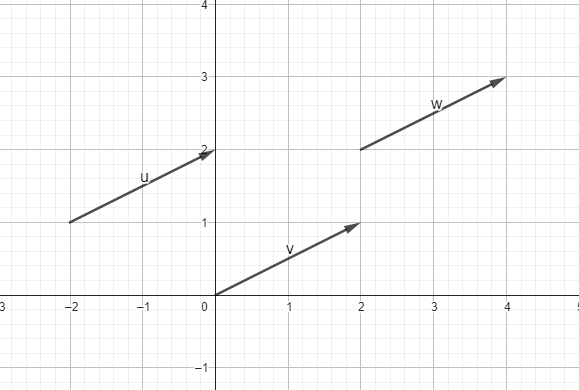
\includegraphics{./images/Vektoren-1-Drei-Vektoren-2022-12-20@16-17-46.png}
        }
    \end{figure}
    Koordinatensystem mit dem Vektor $\vec{v} = \m{2 \\ 1}$ in drei verschiedenen Positionen.

    \subsection{Vektoren 2}
    \begin{figure}[h]
        \centering
        \scalebox{0.5}{
            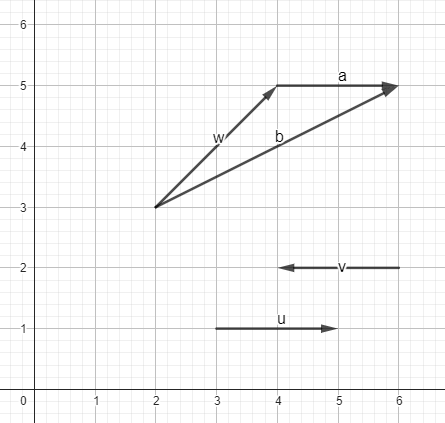
\includegraphics{./images/Vektoren-2-Rechnen-2022-12-19@16-38-25.png}
        }
    \end{figure}
    Multipliziert man den Vektor $\vec{u}$ mit $-1$, erhält man so den Vektor $\vec{v}$.
    Addiert man die Vektoren $\vec{w}$ und $\vec{a}$ resultiert der Vektor $\vec{b}$.

    \newpage

    \subsection{Vektoren 3}
    \begin{figure}[h]
        \centering
        \scalebox{0.5}{
            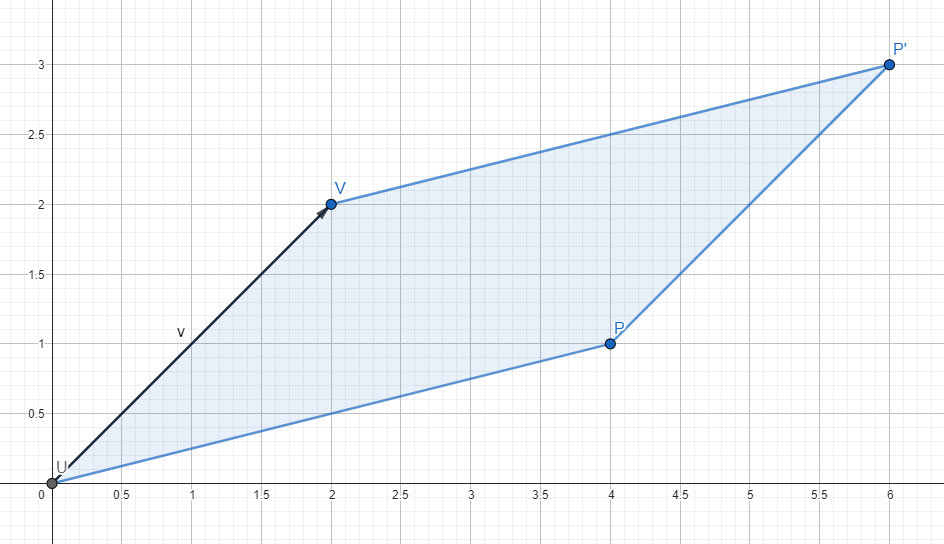
\includegraphics{./images/Vektoren-3-Verschiebung-am-Parallelogramm-2022-12-19@16-30-31.png}
        }
    \end{figure}
    Der Punkt $P$ wird mit dem Vektor $\vec{UV}$ verschoben. Durch das Paralellogramm ergibt sich der neue Punkt $P'$. 
    Der Vektor $\vec{UV}$ ist dabei der Vektor zwischen den beiden Punkten $U$ und $V$ und wird folgendermaßen beschrieben:
    \[
        \begin{split}
            \vec{v} = \vec{UV} = V - U
        \end{split}  
    \]

    \subsection{Vektoren 4}
    \begin{figure}[h]
        \centering
        \scalebox{0.5}{
            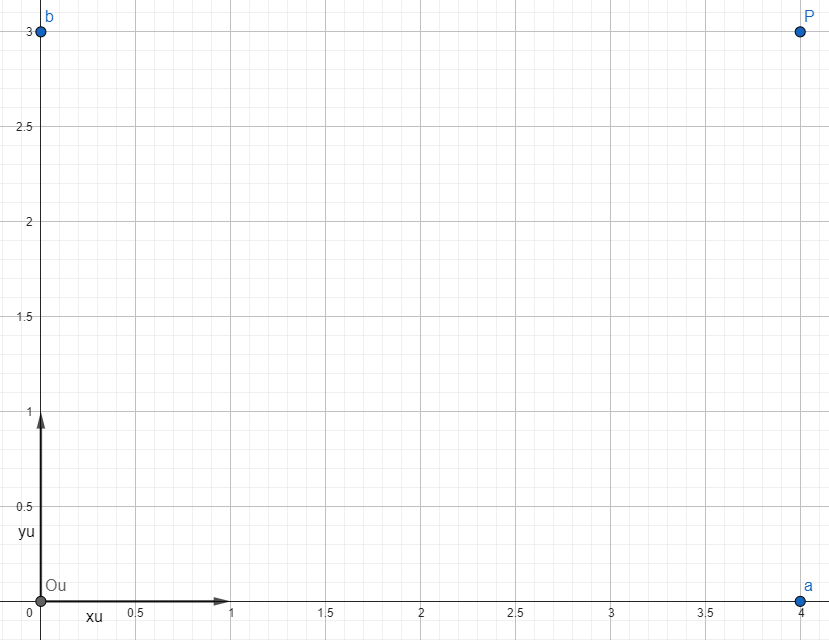
\includegraphics{./images/Vektoren-4-Einheitsvektoren-2022-12-19@17-04-43.png}
        }
    \end{figure}
    Einheitsvektoren $xu$ und $yu$ im Koordinatensystem $U$ mit dem Punkt $P$ und seinen beschreibenden Abschnitten $a$ und $b$.
    
    \newpage


    \subsection{Vektoren 5}
    \begin{figure}[h]
        \centering
        \scalebox{0.5}{
            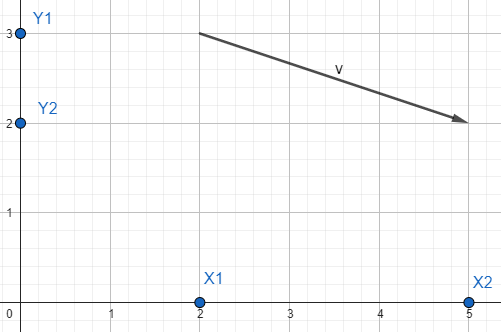
\includegraphics{./images/Vektoren-5-Vektoren-Delta-2022-12-20@16-30-21.png}
        }
    \end{figure}
    Der Vektor $\vec{v}$ wird durch die Differenz des Anfangs- und Endpunktes des Vektors dargestellt.
    \[
        \begin{split}
            \vec{v} = \m{\Delta{x} \\ \Delta{y}} = \m{X2 - X1 \\ Y2 - Y1} = \m{5 - 2 \\ 2 - 3} = \m{3 \\ -1}
        \end{split}  
    \]


    \subsection{Skalarprodukt 1}
    \begin{figure}[h]
        \centering
        \scalebox{0.5}{
            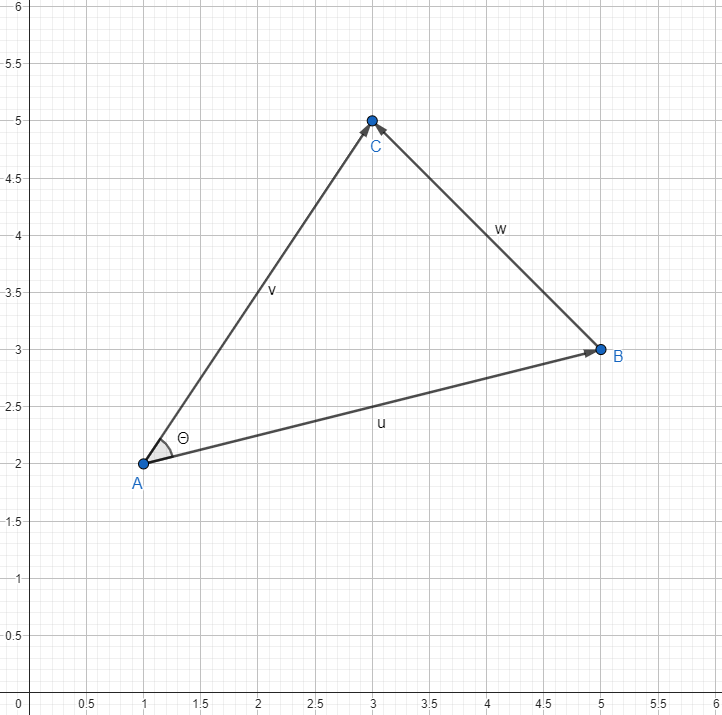
\includegraphics{./images/Skalarprodukt-1-Skizze-2022-12-26@17-27-28.png}
        }
    \end{figure}
    $\vec{w}$ ist der Differenzvektor aus $\vec{v}$ und $\vec{u}$.
    Er hat die Länge $\lVert \vec{v} - \vec{u} \rVert$.
    Der Winkel zwischen $\vec{v}$ und $\vec{u}$ ist $\theta$.

    \newpage

    \subsection{Koordinatentransformation 1}
    \begin{figure}[h]
        \centering
        \scalebox{0.6}{
            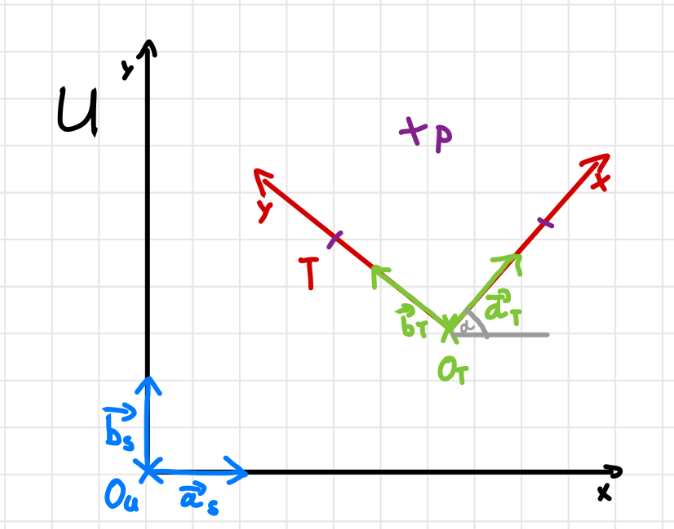
\includegraphics{./images/Trafo-1-2022-12-27@21-54-49.png}
        }
    \end{figure}

    % \subsection{TITEL}
    % \begin{figure}[h]
    %     \centering
    %     \scalebox{0.5}{
    %         
\includegraphics{./images/Mathemann.png}
    %     }
    % \end{figure}

    % ========== Quellen ==========

    \newpage

    \section{Quellen}

    \begin{itemize}
        \item eigene Aufzeichnungen
        \item \url{https://mathe-lok.de/schuelervorlesung-kinematik-von-roboterarmen} (Videos und Folien der 1. und 2. Woche) (Letzter Aufruf: 28.12.2022 @ 18:22:27)
        \item \url{https://www.mathebibel.de/skalarprodukt} (Letzter Aufruf: 26.12.2022 @ 17:23:01)
    \end{itemize}

    % ========== Informationen ==========
    \section{Informationen}

    Die aktuellste Version dieses Dokuments ist unter folgender Internetadresse verfügbar:
    \url{https://github.com/AstragoDEEdu/hausarbeit_robotik_12-2022/blob/main/hausarbeit.pdf}.
    Quelldokumente für Anhänge, sowie Bilder und der Quelltext des Dokuments in \LaTeX{} sind unter folgender Adresse verfügbar:
    \url{https://github.com/AstragoDEEdu/hausarbeit_robotik_12-2022}.

    % ========== Lizenz ==========
    \section{Lizenz}

    Verschiebung von Koordinatensystemen © 2022 von Justus John Michael Seeck ist lizenziert unter Attribution-NonCommercial-ShareAlike 4.0 International.
    Eine Kopie dieser Lizenz ist unter \url{https://creativecommons.org/licenses/by-nc-sa/4.0/} verfügbar.

    Verschiebung von Koordinatensystemen © 2022 by Justus John Michael Seeck is licensed under Attribution-NonCommercial-ShareAlike 4.0 International.
    A copy of this license is available at \url{https://creativecommons.org/licenses/by-nc-sa/4.0/}.

\end{document}